%%%%%%%%%%%%%%%%%%%%%%%%%%%%%%%%%%%%%%%%%%%%%%%%%%%%%%%%%%%%%%%%%%%%%%%%%%%%%%

\documentclass{l3deliverable}

%%%%%%%%%%%%%%%%%%%%%%%%%%%%%%%%%%%%%%%%%%%%%%%%%%%%%%%%%%%%%%%%%%%%%%%%%%%%%%

\usepackage{graphicx}%
\usepackage{url}%

%%%%%%%%%%%%%%%%%%%%%%%%%%%%%%%%%%%%%%%%%%%%%%%%%%%%%%%%%%%%%%%%%%%%%%%%%%%%%%
%% See D1 for an example of how to integrate sub version revision
%% numbers into a LaTeX document.
%

%%%%%%%%%%%%%%%%%%%%%%%%%%%%%%%%%%%%%%%%%%%%%%%%%%%%%%%%%%%%%%%%%%%%%%%%%%%%%%
%% Check these macro values for appropriateness for your own document.

\title{Draft Submission}

\author{Ross Adam \\
        Andrew Gardner \\
        Nicole Kearns \\
        Mamas Nicolaou\\
	Asset Sarsengaliyev\\}

\date{30th January 2013}

\deliverableID{D6}
\project{PSD3 Group Exercise 2}
\team{V}
\version{0.1}

%%%%%%%%%%%%%%%%%%%%%%%%%%%%%%%%%%%%%%%%%%%%%%%%%%%%%%%%%%%%%%%%%%%%%%%%%%%%%%

\begin{document}

%%%%%%%%%%%%%%%%%%%%%%%%%%%%%%%%%%%%%%%%%%%%%%%%%%%%%%%%%%%%%%%%%%%%%%%%%%%%%%

\maketitle

\tableofcontents

\newpage

%%%%%%%%%%%%%%%%%%%%%%%%%%%%%%%%%%%%%%%%%%%%%%%%%%%%%%%%%%%%%%%%%%%%%%%%%%%%%%
%% Standard section for all documents

\section{Introduction}

\subsection{Identification}
System Desgin and Acceptance test plan for internship management system.

\subsection{Related Documentation}

PSD3 Group Exercise Description \url{http://fims.moodle.gla.ac.uk/file.php/128/coursework/psd3-ge-1-rev3278.pdf}\\

Deliverables Template \url{http://fims.moodle.gla.ac.uk/file.php/128/coursework/templates.zip}\\

PSD3 Course Notes \url{http://fims.moodle.gla.ac.uk/file.php/128/lecture-notes/notes-r3275.pdf}\\

\subsection{Purpose and Description of Document}
The purpose of this document is to give a detailed description of our
system desgin and acceptance plan for the internship management system. This report includes a componenet diagram showing the overall architecture of the system, state charts showing the transition between states for the different entities maintained in the system, a set of class diagrams (one for each component in the design), an API specification and an acceptance plan describing the test cases for each component in our design.

\subsection{Document Status and Schedule}

\begin{center}{
\begin{tabular}{|c|c|c|c|}
\hline \textbf{Date} &\textbf{ Change} & \textbf{Version} &\textbf{Author}\\ 
\hline 29/01/13 & Added the state diagrams & 0.1 & Ross\\
\hline 30/01/13 & Added the rationale and description for state diagrams & 0.2 & Ross\\
\hline 30/01/13 & Added the information to the introduction section & 0.3 & Nicole\\ 
\hline 30/01/13 & Added the APIs for the Stores and Authentication & 0.3 & Nicole\\
\hline 30/01/13 & Added the component diagram, and the description and rationale & 0.3 & Nicole, Ross\\
\hline 30/01/13 & Added the Acceptance tests & 0.4 & Asset\\
\hline 30/01/13 & Updated the Acceptance tests & 0.5 & Ross\\
\hline 30/01/13 & Added the APIs for the Advert, Visit, Offer and User Management & 0.6 & Andrew\\
\hline 30/01/13 & Added the Class Diagrams & 0.7 & Mamas\\
\hline 
\end{tabular} }
\end{center}

%%%%%%%%%%%%%%%%%%%%%%%%%%%%%%%%%%%%%%%%%%%%%%%%%%%%%%%%%%%%%%%%%%%%%%%%%%%%%%

\section{Component Diagram}

\begin{center}
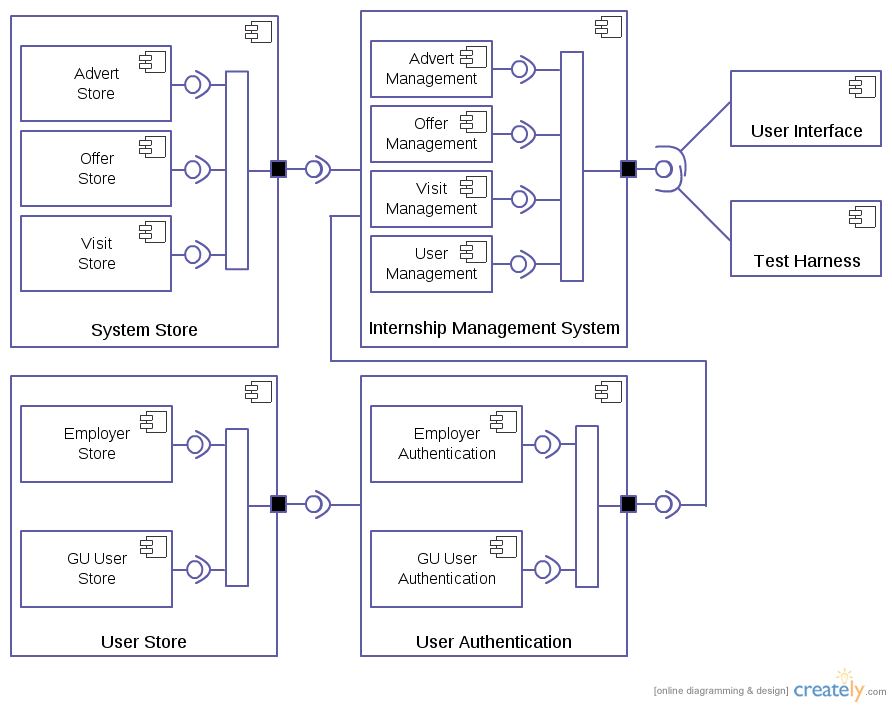
\includegraphics
[scale=0.5]
{img/D6_comp_diagram.png}
\end{center}

\textbf{Rationale}\\
The component diagram was created to illustrate the structural relationship between all components of the internship management system. It also shows the modularity of the different parts of the system.\\

\textbf{Description}\\

The System store is comprised of three separated databases: the Advert Store, Offer Store and the visit store and each of these are drawn together using a facade, which will direct queries to the relevant database. \\

The User Store contains employer store and GU user store. The employer store is a custom database and the GU user store is the myCampus system. Interaction with the myCampus system will be limited to retrieving basic student and staff information.\\

The User Authentication uses two separate components to forward the data to the relevant login system: myCampus or the employer store. \\

The Internship Management System contains several different components that allow the user to interact with the various other components and data stores within the system.\\


%%%%%%%%%%%%%%%%%%%%%%%%%%%%%%%%%%%%%%%%%%%%%%%%%%%%%%%%%%%%%%%%%%%%%%%%%%%%%%

\section{State Diagrams}

\subsection{Rationale}

The following three diagrams were created to illustrate how entities within the application change over time. The three entities are Student, Internship and Advert. These entities were identified by the ``status'' variable in their specification. \\

\subsection{Student}

\textbf{Description} \\
Student was choosen because it displayed 4 distinct states: Approved, Accepted, Withdrawn and Pending. These were identified from the ``View Student Details'' use case. However the finding other use cases to justify this proved difficult as none could be found that implied a change in the Student entity state. Therefore the following diagram was implemented in a manner deemed logical by the team. This is mostly a sub-state diagram encased within a "Not Withdrawn" box. If withdrawn then the sub-state is immediately exited.

\begin{center}
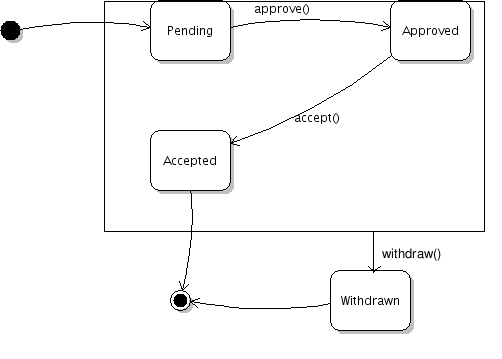
\includegraphics
[scale=0.7]
{img/Student-State.png}
\end{center}

\subsection{Internship}
\textbf{Description}\\
The Internship has two states Pending and Approved. An Internsaddhip starts as either depending on whether it was created by the Course Co-ordinator (Approved) or by a student (Pending). A pending entity can be Approved by the approve method.

\begin{center}
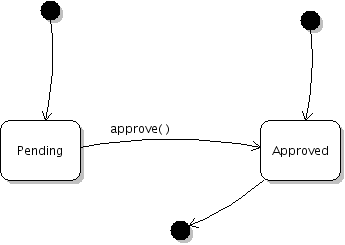
\includegraphics
[scale=0.7]
{img/Internship-state.png}
\end{center}

\subsection{Advert}
\textbf{Description}\\
An Advert can have the following states: Pendign, Not Published and Published. An advert always starts in the pending state, from there it can either become Not Published or Published. It becomes Published if it is deemed acceptable by the Course Co-ordinator and it becomes Not Published if it needs revised. Only a pending or Not Published article can be revised.

\begin{center}
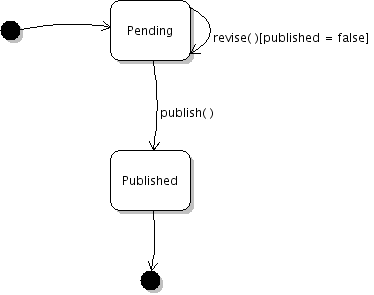
\includegraphics
[scale=0.7]
{img/Advert-State.png}
\end{center}

%%%%%%%%%%%%%%%%%%%%%%%%%%%%%%%%%%%%%%%%%%%%%%%%%%%%%%%%%%%%%%%%%%%%%%%%%%%%%%

\section{Class Diagrams}
\subsection{Advert Store}
\begin{center}
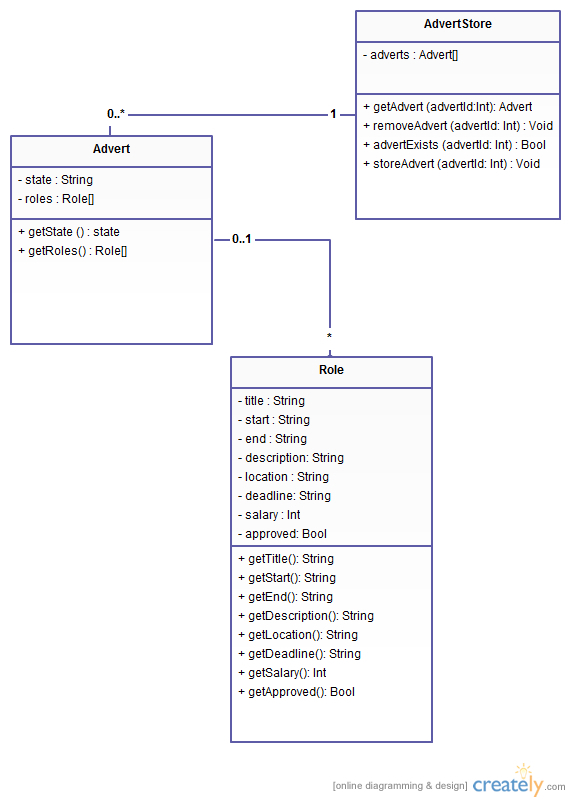
\includegraphics
[scale=0.5]
{img/AdvertStore.jpg}
\end{center}

\subsection{Offer Store}
\begin{center}
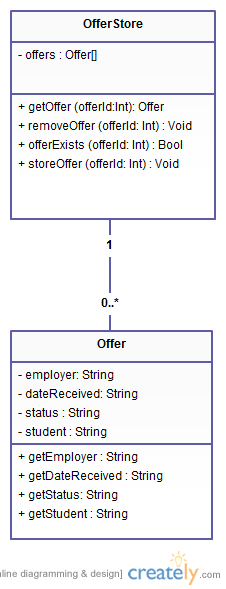
\includegraphics
[scale=0.5]
{img/OfferStore.jpg}
\end{center}

\subsection{Visit Store}
\begin{center}
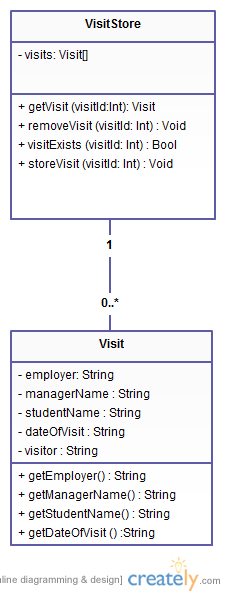
\includegraphics
[scale=0.5]
{img/VisitStore.jpg}
\end{center}

\subsection{Employer Store}
\begin{center}
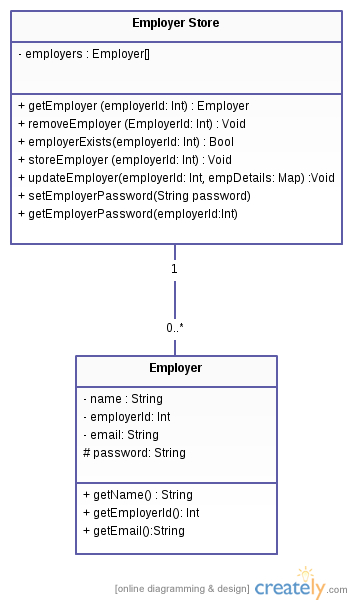
\includegraphics
[scale=0.5]
{img/employerStore.jpg}
\end{center}

\subsection{GU User Store}
\begin{center}
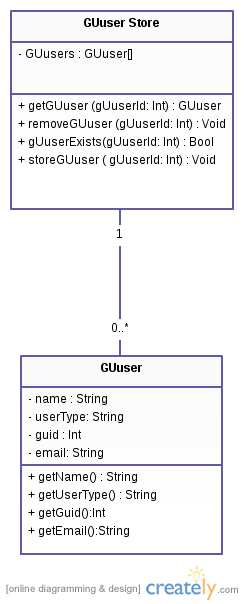
\includegraphics
[scale=0.5]
{img/guuserStore.jpg}
\end{center}

\subsection{Employer Authentication}
\begin{center}
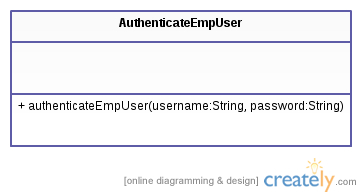
\includegraphics
[scale=0.5]
{img/EmployerAuthentication.jpg}
\end{center}

\subsection{GU User Authentication}
\begin{center}
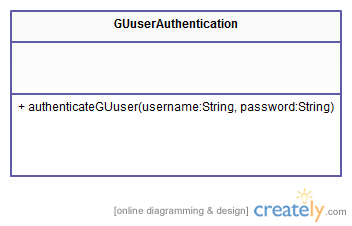
\includegraphics
[scale=0.5]
{img/GUuserAuthentication.jpg}
\end{center}

\subsection{Advert Management}
\begin{center}
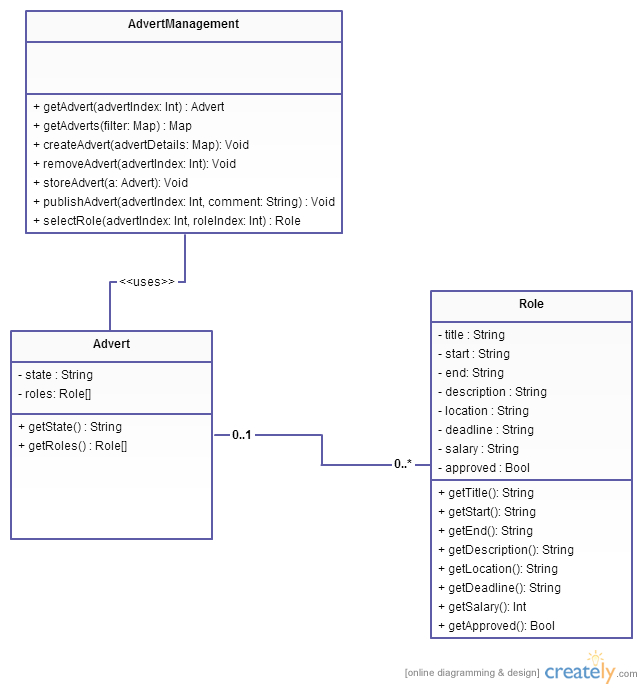
\includegraphics
[scale=0.5]
{img/AdvertManagement.jpg}
\end{center}

\subsection{User Management}
\begin{center}
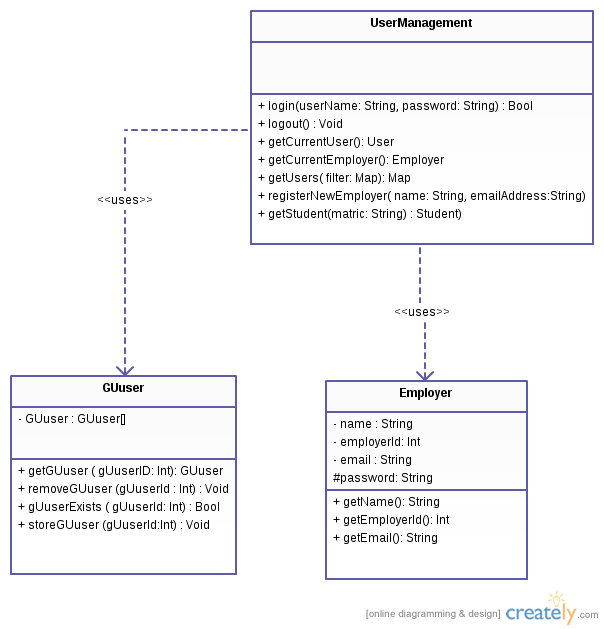
\includegraphics
[scale=0.5]
{img/UserManagement.jpg}
\end{center}

\subsection{Visit Management}
\begin{center}
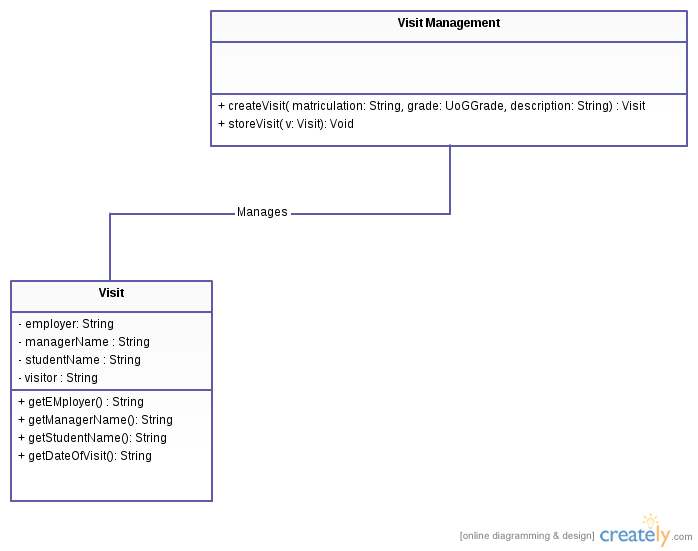
\includegraphics
[scale=0.5]
{img/VisitManagement.jpg}
\end{center}

\subsection{Offer Management}
\begin{center}
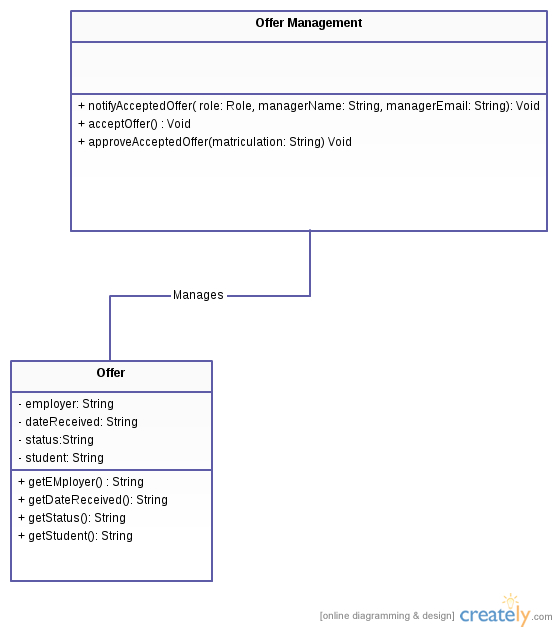
\includegraphics
[scale=0.5]
{img/OfferManagement.jpg}
\end{center}


\subsection{Utility}
\begin{center}
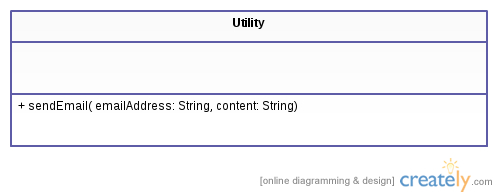
\includegraphics
[scale=0.5]
{img/Utility.jpg}
\end{center}


%%%%%%%%%%%%%%%%%%%%%%%%%%%%%%%%%%%%%%%%%%%%%%%%%%%%%%%%%%%%%%%%%%%%%%%%%%%%%%

\section{API Specification}


\subsection{Advert Store}

\textbf{Method}: Public Advert getAdvert(integer advertId)\\
\textbf{Description}: Gets the advert with the given advert id.\\
\textbf{Parameters}: integer advertId\\
\textbf{Return Type}: Advert\\
\textbf{Pre Condition}: Advert with the given id is available within the system. \\
\textbf{Post Condition}: \\

\textbf{Method}:Public void removeAdvert(integer advertId)\\
\textbf{Description}: The advert with the given advert id is no longer available and removed from the system.\\
\textbf{Parameters}: Integer advertId\\
\textbf{Return Type}: \\
\textbf{Pre Condition}: Advert with the given id is available within the system.\\
\textbf{Post Condition}: Advert is no longer available on the system.\\

\textbf{Method}: Public Boolean advertExists(integer advertId)\\
\textbf{Description}: Checks if a specific advert does exist in the advert store.\\
\textbf{Parameters}: Integer advertId\\
\textbf{Return Type}: Boolean\\
\textbf{Pre Condition}:\\
\textbf{Post Condition}:\\

\textbf{Method}: Public void storeAdvert(integer advertId)\\
\textbf{Description}: Adds a new advert with the given advert id to the advert store. \\
\textbf{Parameters}: Integer advertId\\
\textbf{Return Type}: void\\
\textbf{Pre Condition}: Advert is not already stored in the advert store.\\
\textbf{Post Condition}: Advert is now stored in the advert store.\\

\subsection{Offer Store}

\textbf{Method}: Public Offer getOffer(integer offerId)\\ 
\textbf{Description}: Gets the offer with the given offer id. \\
\textbf{Parameters}: Integer offerId\\
\textbf{Return Type}: Offer\\
\textbf{Pre Condition}: Offer with given id is stored in the system.\\
\textbf{Post Condition}:\\

\textbf{Method}: Public void removeOffer(integer offerId)\\
\textbf{Description}: The offer with the given offer id is removed from the system. \\
\textbf{Parameters}: Integer offerId \\
\textbf{Return Type}: void\\
\textbf{Pre Condition}: offer with the given id is available within the system.\\
\textbf{Post Condition}: offer is no longer stored on the system.\\

\textbf{Method}: Public Boolean offerExists(integer offerId) \\
\textbf{Description}: Checks if a specific offer is stored within the offer store. \\
\textbf{Parameters}: Integer offerId\\
\textbf{Return Type}: Boolean\\
\textbf{Pre Condition}:\\
\textbf{Post Condition}:\\

\textbf{Method}: Public void storeOffer(integer offerId)\\
\textbf{Description}: Adds a new offer with the given offer id to the offer store. \\
\textbf{Parameters}: Integer offerId\\
\textbf{Return Type}: void\\
\textbf{Pre Condition}: offer is not already stored in the offer store.\\
\textbf{Pre Condition}: student notifies course coordinator of internship placement offer.\\
\textbf{Post Condition}: offer is now stored in the offer store.\\

\subsection{Visit Store}

\textbf{Method}: Public Visit getVisit(integer visitId)\\
\textbf{Description}: Gets the visit with the given visit id. \\
\textbf{Parameters}: Integer visitId\\
\textbf{Return Type}: Visit\\
\textbf{Pre Condition}: Visit details are stored in the system.\\
\textbf{Post Condition}:\\

\textbf{Method}: Public void removeVisit(integer advertId)\\
\textbf{Description}: The visit details with the given visit id removed from the system. \\
\textbf{Parameters}: Integer visitId\\
\textbf{Return Type}: void\\
\textbf{Pre Condition}: visit details with the given id are available within the system.\\
\textbf{Post Condition}: visit details are no longer available on the system.\\

\textbf{Method}: Public Boolean visitExists(integer adverted)\\
\textbf{Description}: Checks if a specific visit does is stored in the visit store. \\
\textbf{Parameters}: Integer visitId\\
\textbf{Return Type}: Boolean\\
\textbf{Pre Condition}:\\
\textbf{Post Condition}:\\

\textbf{Method}: Public void storeVisit(integer visitId) \\
\textbf{Description}:  adds the details of a new visit with the given visit id to the visit store.\\
\textbf{Parameters}: Integer visitId\\
\textbf{Return Type}: void\\
\textbf{Pre Condition}: Visit is not already stored in the visit store.\\
\textbf{Post Condition}: visit is now stored in the visit store.\\

\subsection{Employer Store}

\textbf{Method}: Public Employer getEmployer(integer employerId)\\
\textbf{Description}: Gets the employer with the given employer id.\\
\textbf{Parameters}:  Integer employerId\\
\textbf{Return Type}: Employer\\
\textbf{Pre Condition}: Employer with given employerId is available in the system.\\
\textbf{Post Condition}:\\

\textbf{Method}: Public void removeEmployer(integer employerId) \\
\textbf{Description}: will remove the employer with the specified id from the system, meaning that they can no longer log in to the system\\
\textbf{Parameters}: Integer empoyerId\\
\textbf{Return Type}: void\\
\textbf{Pre Condition}: The employer is stored in the Employer Store\\
\textbf{Post Condition}: The employer details are no longer available/stored.\\

\textbf{Method}: Public boolean employerExists(integer employerId) \\
\textbf{Description}: checks if a specific employer is stored within the employer store.\\
\textbf{Parameters}: Integer employerId\\
\textbf{Return Type}: Boolean\\
\textbf{Pre Condition}:\\
\textbf{Post Condition}:\\

\textbf{Method}: Public void storeEmployer(integer employerId) \\
\textbf{Description}:  Adds a new Employer with the given Employer id to the Employer store.\\
\textbf{Parameters}: Integer employerId\\
\textbf{Return Type}: void\\
\textbf{Pre Condition}: employer with the specified id does not exist in the employer store.\\
\textbf{Post Condition}: Employer is stored in the employer store.\\

\textbf{Method}: Public void updateEmployer(integer employerID, Map empDetails)\\
\textbf{Description}: updates the specified details for the employer with the given employerId.\\
\textbf{Parameters}: Integer employerId, Map empDetails\\
\textbf{Return Type}: void\\
\textbf{Pre Condition}: employer is already stored in the system.\\
\textbf{Post Condition}: The specified details are updated in the system.\\


\textbf{Method}: Public void setEmployerPassword(String password) \\
\textbf{Description}: Allows the Employer to set up a new password.\\
\textbf{Parameters}: String password\\
\textbf{Return Type}: void\\
\textbf{Pre Condition}: Employer with given id is available in the system.\\
\textbf{Post Condition}: New password is now set to the String passed in.\\

\textbf{Method}: Public String getEmployerPassword(Integer employerId) \\
\textbf{Description}: Will provide the user with the password for the specific employer.\\
\textbf{Parameters}: Integer employerId\\
\textbf{Return Type}: String \\
\textbf{Pre Condition}: Employer is available in the system.\\
\textbf{Post Condition}:\\

\subsection{GU User Store}

\textbf{Method}: Public GUuser getGUuser(integer GUuserId)\\
\textbf{Description}: Gets the employer with the given GUID.\\
\textbf{Parameters}: Integer GUuserId\\
\textbf{Return Type}: GUuser\\
\textbf{Pre Condition}: GUuser with given GUuserId is available in the system.\\
\textbf{Post Condition}:\\

\textbf{Method}: Public void removeGUuser(integer GuuserId)\\
\textbf{Description}: Will remove the GU user with the specified id from the system, meaning that they can no longer log in to the system.
\\
\textbf{Parameters}: Integer GUuserId\\
\textbf{Return Type}: void\\
\textbf{Pre Condition}: GU user details are stored in the GU user store\\
\textbf{Post Condition}: User details are no longer available in the GU user store\\

\textbf{Method}: Public boolean GUuserExists(integer GuuserId)\\
\textbf{Description}: Checks if a specific GU user is stored within the GU user store.\\
\textbf{Parameters}: Integer GUuserId\\
\textbf{Return Type}: Boolean\\
\textbf{Pre Condition}:\\
\textbf{Post Condition}:\\

\textbf{Method}: Public void storeGUuser (integer GUuserId)\\
\textbf{Description}: Adds a new GU user with the given GUuser id to the GU user store.\\
\textbf{Parameters}: Integer GUuserId\\
\textbf{Return Type}: void\\
\textbf{Pre Condition}: No user with the given id is stored in the GU user store\\
\textbf{Post Condition}: GU user is stored in the GU user store.\\

\subsection{Employer Authentication}

\textbf{Method}: Public void authenticateEmpUser(String username, String password)\\
\textbf{Description}: Checks that the username and password for the user are correct.\\
\textbf{Parameters}: String username, String password\\
\textbf{Return Type}: void\\
\textbf{Pre Condition}: Employer user is not logged in to the system.\\
\textbf{Post Condition}: Employer is logged into the system.\\

\subsection{GU User Authentication}

\textbf{Method}: Public void authenticateGUuser(String username, String password)\\
\textbf{Description}: Checks that the username and password for the user are correct. \\
\textbf{Parameters}: String username, String password\\
\textbf{Return Type}: void\\
\textbf{Pre Condition}: GU user is not logged in to the system.\\
\textbf{Post Condition}: GU user is logged into the system.\\


\subsection{Advert Management Component}
\textbf{Method}: public Advert getAdvert( Integer advertisementIndex )\\
\textbf{Description}: Returns advert specified by its index\\
\textbf{Parameters}: Integer advertisementIndex\\
\textbf{Return Type}: Advert\\
\textbf{Pre Condition}: Advert must be stored in system\\
\textbf{Post Condition}:\\

\textbf{Method}: public Map getAdverts( Map filter )\\
\textbf{Description}: Returns set of adverts, filtered by mapped options\\
\textbf{Parameters}: Map filter\\
\textbf{Return Type}: Map\\
\textbf{Pre Condition}: At least one advert stored in system\\
\textbf{Post Condition}:\\

\textbf{Method}: public Advert createAdvert( Map advertDetails )\\
\textbf{Description}: Creates \& returns advert\\
\textbf{Parameters}: Map advertDetails\\
\textbf{Return Type}: Advert \\
\textbf{Pre Condition}:\\
\textbf{Post Condition}:\\

\textbf{Method}: public void removeAdvert( Integer advertIndex )\\
\textbf{Description}: Removes advertisment from system\\
\textbf{Parameters}: Integer advertIndex \\
\textbf{Return Type}: void \\
\textbf{Pre Condition}: Advertisement must be in system \\
\textbf{Post Condition}: Advertisement no longer present in system\\

\textbf{Method}: public void storeAdvertisement( Advert a )\\
\textbf{Description}: Stores advertisement in system\\
\textbf{Parameters}: Advert a\\
\textbf{Return Type}: void\\
\textbf{Pre Condition}:\\
\textbf{Post Condition}: Advert stored in system\\

\textbf{Method}: public void publishAdvertisement ( Integer advertIndex, String comment )\\
\textbf{Description}: Makes advertisement visible to students \& sends comment to employer by E-Mail\\
\textbf{Parameters}: Integer advertIndex, String comment\\
\textbf{Return Type}: void\\
\textbf{Pre Condition}: Advertisement must be in system \& be unpublished\\
\textbf{Post Condition}: Advertisment is now visible to students\\

\textbf{Method}: public Role selectRole( Integer advertIndex, Integer roleIndex )\\
\textbf{Description}: Returns role for an advertisement, both specified by index\\
\textbf{Parameters}: Integer advertIndex, Integer roleIndex\\
\textbf{Return Type}: Role\\
\textbf{Pre Condition}: Advert \& role must be in system\\
\textbf{Post Condition}:\\


\subsection{User Management Component}

\textbf{Method}: public boolean login( String userName, String password )\\
\textbf{Description}: Logs user into the system\\
\textbf{Parameters}: String userName, String password\\
\textbf{Return Type}: boolean\\
\textbf{Pre Condition}: User exists on system \& not currently logged in\\
\textbf{Post Condition}: Set as current user\\

\textbf{Method}: public void logout( )\\
\textbf{Description}: Logs user out of the system\\
\textbf{Parameters}:\\
\textbf{Return Type}: void\\
\textbf{Pre Condition}: User currently logged in\\
\textbf{Post Condition}: Un-sets current user\\

\textbf{Method}: public User getCurrentUser( )\\
\textbf{Description}: Returns currently logged in user\\
\textbf{Parameters}:\\
\textbf{Return Type}: User\\
\textbf{Pre Condition}: User currently logged in\\
\textbf{Post Condition}:\\

\textbf{Method}: public User getCurrentEmployer( )\\
\textbf{Description}: Returns currently selected employer\\
\textbf{Parameters}:\\
\textbf{Return Type}: Employer\\
\textbf{Pre Condition}: An employer must be selected\\
\textbf{Post Condition}:\\

\textbf{Method}: public Map getUsers( Map filter )\\
\textbf{Description}: Returns set of users, filtered by mapped options\\
\textbf{Parameters}: Map filter\\
\textbf{Return Type}: Map\\
\textbf{Pre Condition}: At least one user in system\\
\textbf{Post Condition}:\\

\textbf{Method}: public Employer registerNewEmployee( String name, String emailAddress )\\
\textbf{Description}: Returns employer after setting up an account for them\\
\textbf{Parameters}: String name, String emailAddress\\
\textbf{Return Type}: Employer\\
\textbf{Pre Condition}: Employer shouldn't exist on system\\
\textbf{Post Condition}: Employer has account on system\\

\textbf{Method}: public Student getStudent( String matric )\\
\textbf{Description}: Returns student specified by matric\\
\textbf{Parameters}: String matric\\
\textbf{Return Type}: Student\\
\textbf{Pre Condition}: Student must exist in system\\
\textbf{Post Condition}:\\

\textbf{Method}: public void notifyAcceptedOffer( Role role, String managerName, String managerEmail )\\
\textbf{Description}: Notifies coordinator of accepted offer by E-Mail\\
\textbf{Parameters}: Role role, String managerName, String managerEmail\\
\textbf{Return Type}: void\\
\textbf{Pre Condition}: Student must be logged in\\
\textbf{Post Condition}:\\

\subsection{Offer Management}
\textbf{Method}: public void acceptOffer( ) \\
\textbf{Description}: TODO?\\
\textbf{Parameters}: TODO?\\
\textbf{Return Type}: TODO?\\
\textbf{Pre Condition}: TODO?\\
\textbf{Post Condition}: TODO?\\

\textbf{Method}: public void approveAcceptedOffer( String matriculation )\\
\textbf{Description}: Approves offer most recently accepted by student with this matriculation id\\
\textbf{Parameters}: String matriculation\\
\textbf{Return Type}: void\\
\textbf{Pre Condition}: Student needs to have accepted at least one offer \\
\textbf{Post Condition}:\\

\subsection{Visit Management}
\textbf{Method}: public Visit createVisit( String matriculation, UoGGrade grade, String description )\\
\textbf{Description}: Creates and returns a visit\\
\textbf{Parameters}: String matriculation, UoGGrade grade, String description\\
\textbf{Return Type}: Visit\\
\textbf{Pre Condition}: Student must exist on system\\
\textbf{Post Condition}:\\

\textbf{Method}: public void storeVisit( Visit v )\\
\textbf{Description}: Stores visit in system\\
\textbf{Parameters}: Visit v\\
\textbf{Return Type}: void\\
\textbf{Pre Condition}:\\
\textbf{Post Condition}:\\

\subsection{Utility Component}
\textbf{Method}: public void sendEmail( String emailAddress, String content ) \\
\textbf{Description}: Sends an E-Mail containing content to emailAddress\\
\textbf{Parameters}: String emailAddress, String content\\
\textbf{Return Type}: void\\
\textbf{Pre Condition}:\\
\textbf{Post Condition}:\\



%%%%%%%%%%%%%%%%%%%%%%%%%%%%%%%%%%%%%%%%%%%%%%%%%%%%%%%%%%%%%%%%%%%%%%%%%%%%%%

\section{Acceptance Tests}

Before the Internship Management System can be deployed we must create
several acceptance tests to ensure that the program covers all the
requirements from the specification. These acceptance tests are not
designed to identify bugs but to ensure that the user can interact
with the application and use it's advertised functions.\\

\begin{tabular}{|c|c|}
\hline \textbf{Identifier} & T.C.5.1.1\\
\hline \textbf{Use case} & Login \\
\hline \textbf{Scenario} & Logging in as a course coordinator \\
\hline \textbf{Set up} & System initialised with default parameters\\
\hline \textbf{Includes} & none\\
\hline \textbf{Procedure} & Not defined yet\\
\hline \textbf{Inputs} & User = «ccadmin», password=pass\\
\hline \textbf{Outputs} & User set from guest to ccadmin \\
\hline
\end{tabular}

\begin{tabular}{|c|c|}
\hline \textbf{Identifier} & T.C.5.1.2 \\
\hline \textbf{Use case} & Login\\
\hline \textbf{Scenario} & Invalid login/password\\
\hline \textbf{Set up} & System initialised with default parameters\\
\hline \textbf{Includes} & none\\
\hline \textbf{Procedure} & Not defined yet\\
\hline \textbf{Inputs} & User = «ccadmin», password=pass1\\
\hline \textbf{Outputs} & User has not changed to ccadmin or gained
access to admin features \\
\hline
\end{tabular}

\begin{tabular}{|c|c|}
\hline \textbf{Identifier} & T.C.5.1.3\\
\hline \textbf{Use case} & Login \\
\hline \textbf{Scenario} & Logging in as a student\\
\hline \textbf{Set up} & System initialised with default parameters\\
\hline \textbf{Includes} & none\\
\hline \textbf{Procedure} & not defined yet\\
\hline \textbf{Inputs} & User = «2060267s», password=password\\
\hline \textbf{Outputs} & User has changed to student\\
\hline
\end{tabular}

\begin{tabular}{|c|c|}
\hline \textbf{Identifier} & T.C.5.1.4 \\
\hline \textbf{Use case} & Login \\
\hline \textbf{Scenario} & Logging in as a company\\
\hline \textbf{Set up} & System initilised with default parameters and logged in\\
\hline \textbf{Includes} & T.C.5.7.1\\
\hline \textbf{Procedure} & Not defined yet\\
\hline \textbf{Inputs} & User = «Google», password=Mypassword1998\\
\hline \textbf{Outputs} & User has changed to company\\
\hline
\end{tabular}

The above Tests cover the different user types logging in with both
invalid and valid passwords.\\ 

\begin{tabular}{|c|c|}
\hline \textbf{Identifier} & T.C.5.2.1 \\
\hline \textbf{Use case} & Logout \\
\hline \textbf{Scenario} & Logging out\\
\hline \textbf{Set up} & System initilised with default parameters and logged in\\
\hline \textbf{Includes} & T.C.5.1.1/T.C.5.1.3/T.C.5.1.4 (logged in as a registered user)\\
\hline \textbf{Procedure} & Not defined yet\\
\hline \textbf{Inputs} & logout\\
\hline \textbf{Outputs} & User has changed to guest\\
\hline
\end{tabular}

\begin{tabular}{|c|c|}
\hline \textbf{Identifier} & T.C.5.3.1 \\
\hline \textbf{Use case} & View internship list\\
\hline \textbf{Scenario} & Viewing approved internships\\
\hline \textbf{Set up} & System initilised with default parameters and logged in\\
\hline \textbf{Includes} & T.C.5.1.1/T.C.5.1.3 (logged in as a member of university)\\
\hline \textbf{Procedure} & Not defined yet\\
\hline \textbf{Inputs} & view\\
\hline \textbf{Outputs} & All approved internship lists are shown\\
\hline
\end{tabular}

\begin{tabular}{|c|c|}
\hline \textbf{Identifier} & T.C.5.3.2 \\
\hline \textbf{Use case} & View internship list\\
\hline \textbf{Scenario} & Show unapproved intershnips\\
\hline \textbf{Set up} & System initilised with default parameters and logged in\\
\hline \textbf{Includes} &T.C.5.1.1 (course coordinator), T.C.5.5.1(submitted ads)\\
\hline \textbf{Procedure} & Not defined yet\\
\hline \textbf{Inputs} & View unapproved\\
\hline \textbf{Outputs} & All unapproved internship lists are shown\\
\hline
\end{tabular}

\begin{tabular}{|c|c|}
\hline \textbf{Identifier} & T.C.5.4.1 \\
\hline \textbf{Use case} & Edit internship\\
\hline \textbf{Scenario} & Primary\\
\hline \textbf{Set up} & Logged in as a course coordinator\\
\hline \textbf{Includes} & T.C.5.1.1, T.C.5.6.1 (ad details shown, course coordinator)\\
\hline \textbf{Procedure} & Not defined yet \\
\hline \textbf{Inputs} & New description\\
\hline \textbf{Outputs} & Internship is updated\\
\hline
\end{tabular}

\begin{tabular}{|c|c|}
\hline \textbf{Identifier} & T.C.5.5.1\\
\hline \textbf{Use case} & Submit internship\\
\hline \textbf{Scenario} & Primary\\
\hline \textbf{Set up} & Logged in as a company\\
\hline \textbf{Includes} & T.C.5.1.4 (company login)\\
\hline \textbf{Procedure} & Not defined yet\\
\hline \textbf{Inputs} & Internship details\\
\hline \textbf{Outputs} & Email sent to course coordinator\\
\hline
\end{tabular}

\begin{tabular}{|c|c|}
\hline \textbf{Identifier} & T.C.5.6.1\\
\hline \textbf{Use case} & View advertisement detail\\
\hline \textbf{Scenario} & Primary\\
\hline \textbf{Set up} & System initilised with default parameters and logged in\\
\hline \textbf{Includes} & T.C.5.1.1 T.C.5.1.3 T.C.5.1.4 T.C.5.5.1\\
\hline \textbf{Procedure} & Not defined yet\\
\hline \textbf{Inputs} & Select internship\\
\hline \textbf{Outputs} & Selected internship details are shown\\
\hline
\end{tabular}

\begin{tabular}{|c|c|}
\hline \textbf{Identifier} & T.C.5.7.1\\
\hline \textbf{Use case} & Register employer\\
\hline \textbf{Scenario} & Employer is registered\\
\hline \textbf{Set up} & System initilised with default parameters\\
\hline \textbf{Includes} & none\\
\hline \textbf{Procedure} & Not defined yet\\
\hline \textbf{Inputs} & Valid employer details\\
\hline \textbf{Outputs} & Details sent to course coordinator\\
\hline
\end{tabular}

\begin{tabular}{|c|c|}
\hline \textbf{Identifier} & T.C.5.7.2\\
\hline \textbf{Use case} & Register employer\\
\hline \textbf{Scenario} & Invalid details\\
\hline \textbf{Set up} & System initilised with default parameters\\
\hline \textbf{Includes} & none\\
\hline \textbf{Procedure} & Not defined yet\\
\hline \textbf{Inputs} & Invalid/missing employer details\\
\hline \textbf{Outputs} & Warning message is shown with error details\\
\hline
\end{tabular}

\begin{tabular}{|c|c|}
\hline \textbf{Identifier} & T.C.5.8.1\\
\hline \textbf{Use case} & View advertisement summary\\
\hline \textbf{Scenario} & Primary\\
\hline \textbf{Set up} & System initilised with published advertisements\\
\hline \textbf{Includes} & T.C.5.9.1 T.C.5.1.1\\
\hline \textbf{Procedure} & Not defined yet\\
\hline \textbf{Inputs} & View ads\\
\hline \textbf{Outputs} & Advertisement summary is shown\\
\hline
\end{tabular}

\begin{tabular}{|c|c|}
\hline \textbf{Identifier} & T.C.5.9.1\\
\hline \textbf{Use case} & Review/publish advert\\
\hline \textbf{Scenario} & Primary\\
\hline \textbf{Set up} & System initilised with unpublished advertisements\\
\hline \textbf{Includes} & T.C.5.1.1 T.C.5.5.1\\
\hline \textbf{Procedure} & Not defined yet\\
\hline \textbf{Inputs} & Unpublished ad\\
\hline \textbf{Outputs} & Ad is published, company is notified\\
\hline
\end{tabular}

\begin{tabular}{|c|c|}
\hline \textbf{Identifier} & T.C.5.9.2\\
\hline \textbf{Use case} & Review/publish advert\\
\hline \textbf{Scenario} & Secondary\\
\hline \textbf{Set up} & System initilised with unpublished advertisements\\
\hline \textbf{Includes} & T.C.5.1.1 T.C.5.5.1\\
\hline \textbf{Procedure} & Not defined yet\\
\hline \textbf{Inputs} & Unpublished ad\\
\hline \textbf{Outputs} & Ad is not published, company is notified\\
\hline
\end{tabular}

\begin{tabular}{|c|c|}
\hline \textbf{Identifier} & T.C.5.10.1\\
\hline \textbf{Use case} & Notify course coordinator\\
\hline \textbf{Scenario} & primary\\
\hline \textbf{Set up} & Internship details are filled in, logged as a student\\
\hline \textbf{Includes} & T.C.5.1.3\\
\hline \textbf{Procedure} & Not defined yet\\
\hline \textbf{Inputs} & Internship details\\
\hline \textbf{Outputs} & Email sent to course coordinator for approval\\
\hline
\end{tabular}

\begin{tabular}{|c|c|}
\hline \textbf{Identifier} & T.C.5.10.2\\
\hline \textbf{Use case} & Notify course coordinator\\
\hline \textbf{Scenario} & secondary\\
\hline \textbf{Set up} & logged as a student\\
\hline \textbf{Includes} & T.C.5.1.3\\
\hline \textbf{Procedure} & Not defined yet\\
\hline \textbf{Inputs} & Missing/invalid Internship details\\
\hline \textbf{Outputs} & Warning message is shown\\
\hline
\end{tabular}

\begin{tabular}{|c|c|}
\hline \textbf{Identifier} & T.C.5.11.1\\
\hline \textbf{Use case} & Approve advert\\
\hline \textbf{Scenario} & Approving internship\\
\hline \textbf{Set up} & logged as a course coordinator\\
\hline \textbf{Includes} & T.C.5.1.1 T.C.5.11.1\\
\hline \textbf{Procedure} & Not defined yet\\
\hline \textbf{Inputs} & Approve\\
\hline \textbf{Outputs} & Internship approved in student details\\
\hline
\end{tabular}

\begin{tabular}{|c|c|}
\hline \textbf{Identifier} & T.C.5.11.2\\
\hline \textbf{Use case} & Approve advert\\
\hline \textbf{Scenario} & Disapproving internship\\
\hline \textbf{Set up} & logged as a course coordinator\\
\hline \textbf{Includes} & T.C.5.1.1 T.C.5.11.1\\
\hline \textbf{Procedure} & Not defined yet\\
\hline \textbf{Inputs} & Disapprove\\
\hline \textbf{Outputs} & Internship disapproved in student details\\
\hline
\end{tabular}

These test cases will be implemented using the JUnit class within
Java. 

\end{document}
